
%---------------------------------------------------------------
% The "*" following chapter or section commands omits chapter/
% section numbers.  It also does not include the chapter/section
% in the table of contents -- the \addcontentsline can be used
% to manually force its entry.
%---------------------------------------------------------------

\chapter*{}
\addcontentsline{toc}{chapter}{Appendix}

% This command creates the Appendix page without a page number
\thispagestyle{empty}

\vbox to 3.75in{}
\begin{center}
{\textbf{APPENDICES}}
\vfill
\end{center}

\addtocounter{page}{-1}
\newpage


\chapter*{}\label{Ap1}
\begin{center}
APPENDIX I
\end{center}

\begin{figure}[!htbp]
	\centering
	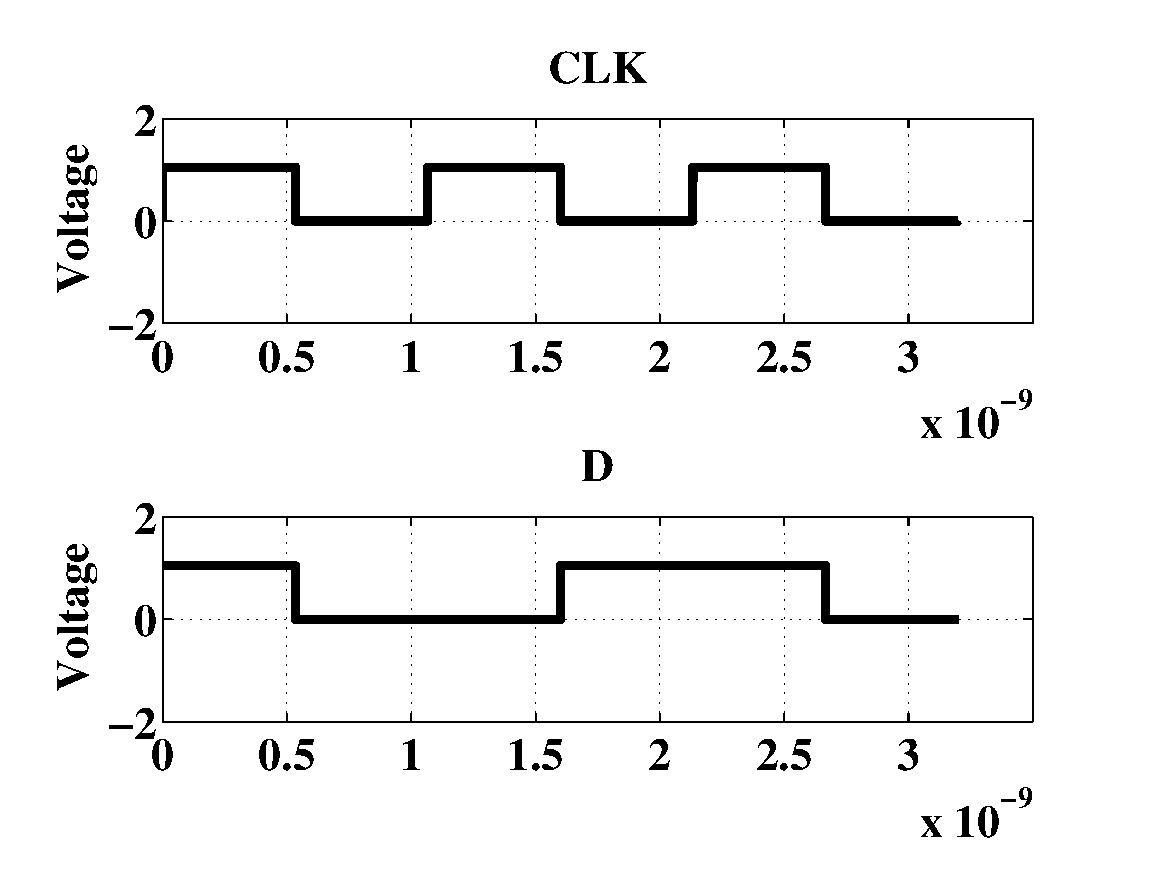
\includegraphics[width=0.55\linewidth]{Figures/WavePlots/CLKD.eps}
	%where an .eps filename suffix will be assumed under latex, 
	%and a .pdf suffix will be assumed for pdflatex; or what has been declared
	%via \DeclareGraphicsExtensions.
	\caption{Waveforms for CLK and D.}
	\label{fig:CLK}
\end{figure}

\begin{figure}[!htbp]
	\centering
	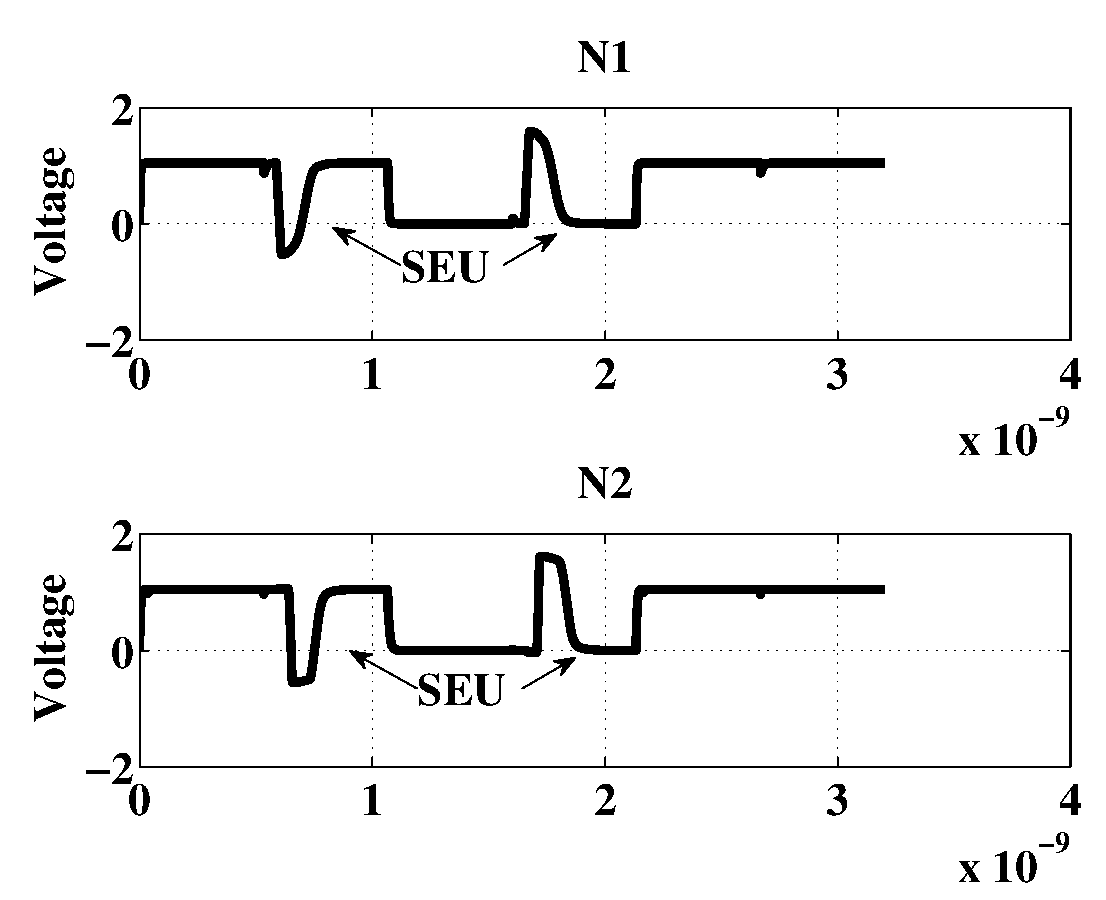
\includegraphics[width=0.5\linewidth]{Figures/WavePlots/n1n2.eps}
	\caption{Node pair n1 and n2 upset and recovery.}
	\label{fig:n1n2}
\end{figure}

\begin{figure}[!htbp]
	\centering
	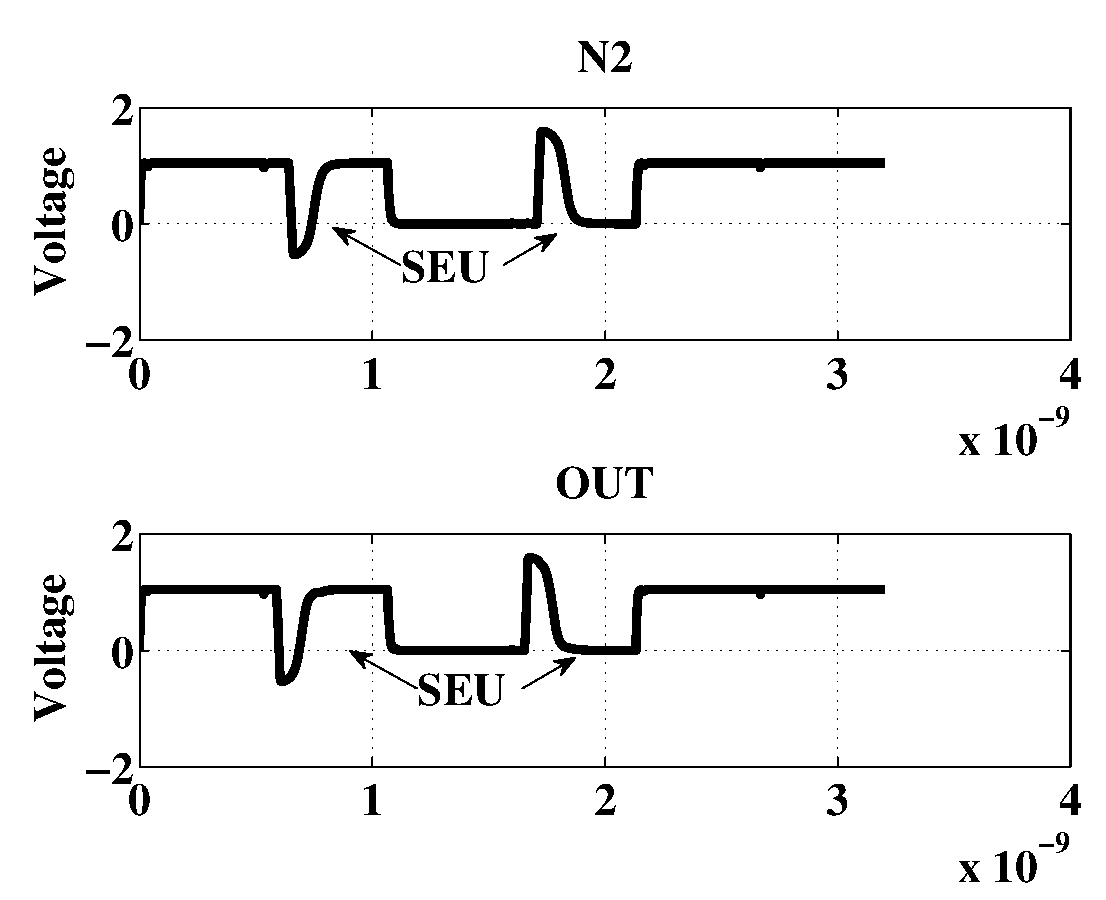
\includegraphics[width=0.5\linewidth]{Figures/WavePlots/n2out.eps}
	\caption{Node pair n2 and out upset and recovery.}
	\label{fig:n2out}
\end{figure}

\begin{figure}[!htbp]
	\centering
	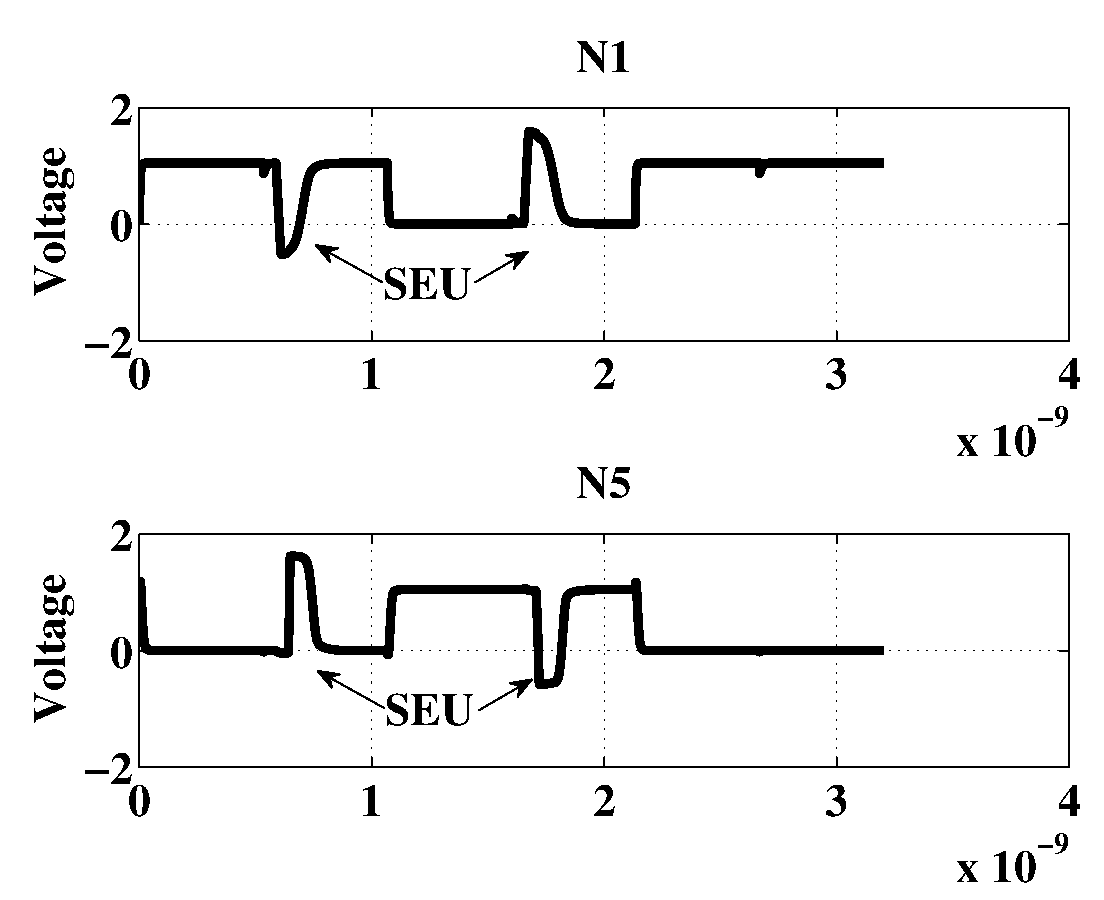
\includegraphics[width=0.5\linewidth]{Figures/WavePlots/n1n5.eps}
	\caption{Node pair n1 and n5 upset and recovery.}
	\label{fig:n1n5}
\end{figure}

\begin{figure}[!htbp]
	\centering
	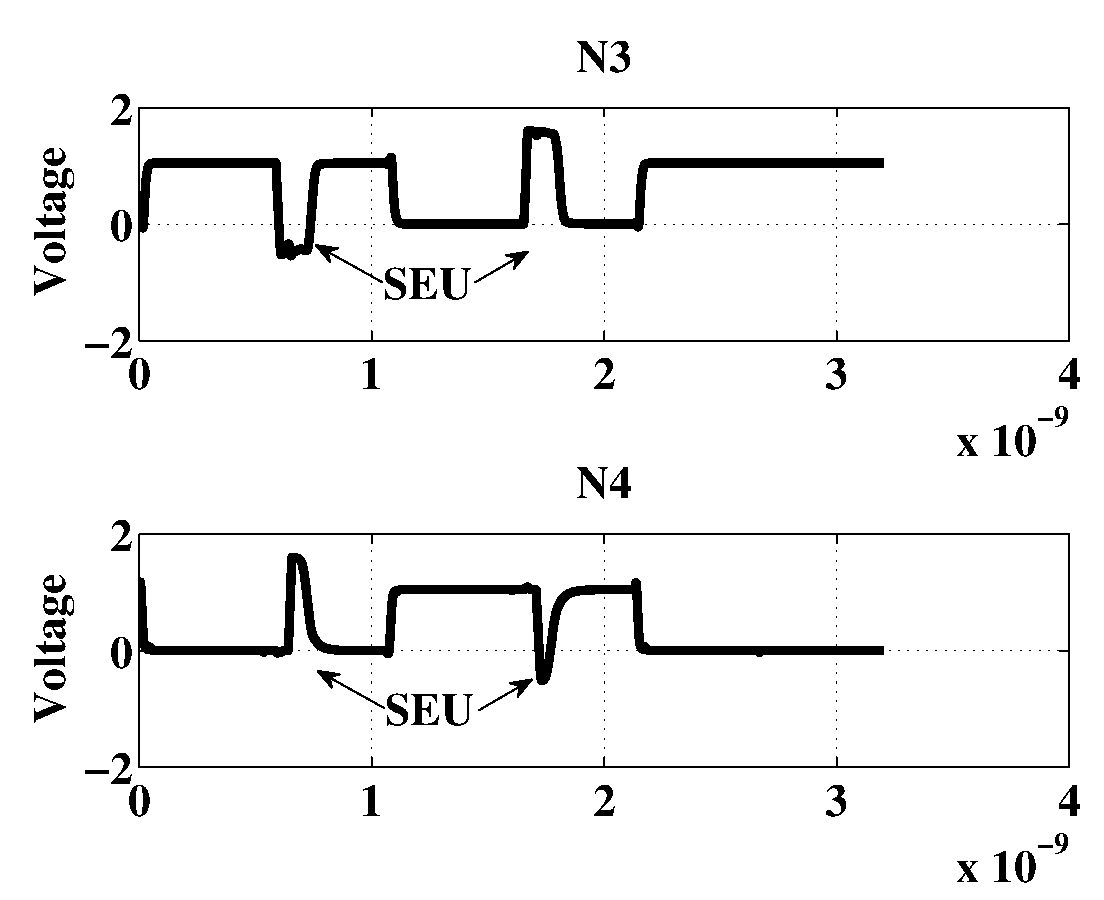
\includegraphics[width=0.5\linewidth]{Figures/WavePlots/n3n4.eps}
	\caption{Node pair n3 and n4 upset and recovery.}
	\label{fig:n3n4}
\end{figure}

\begin{figure}[!htbp]
	\centering
	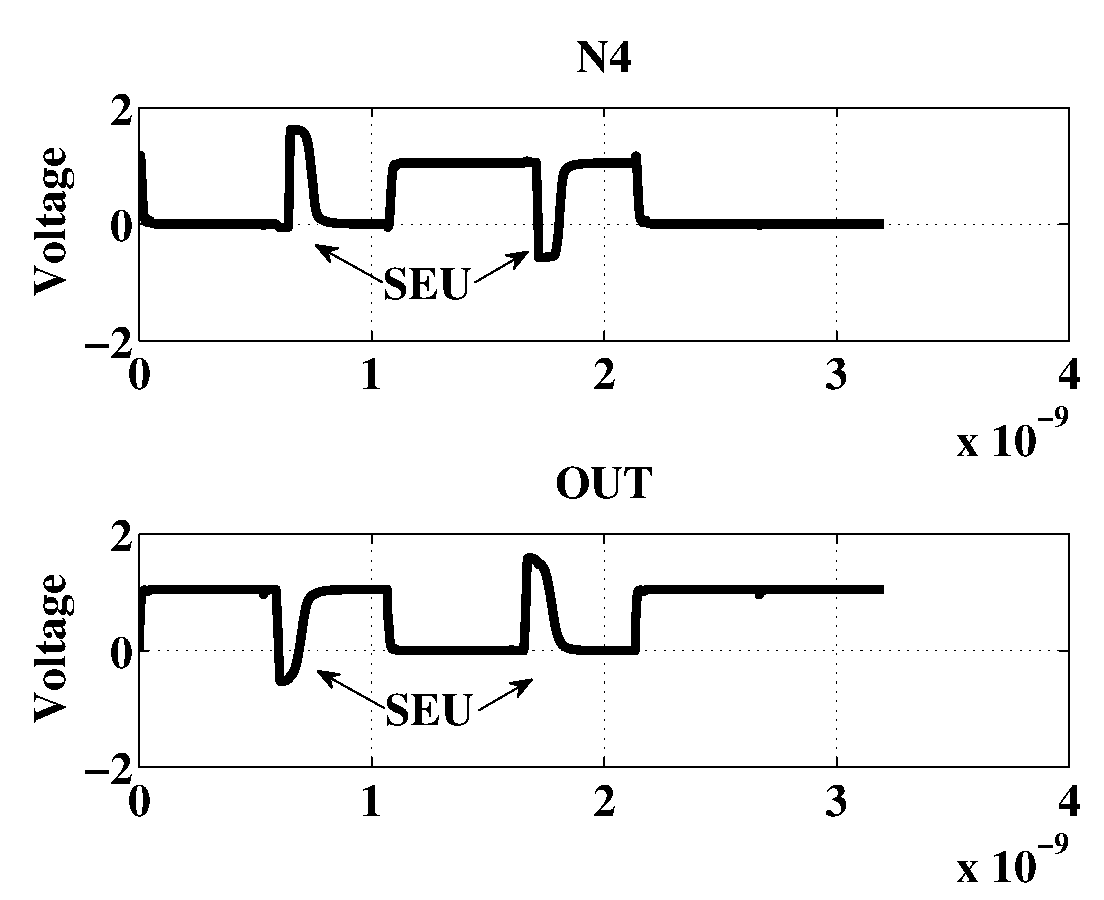
\includegraphics[width=0.5\linewidth]{Figures/WavePlots/n4out.eps}
	\caption{Node pair n4 and out upset and recovery.}
	\label{fig:n4out}
\end{figure}

\begin{figure}[!htbp]
	\centering
	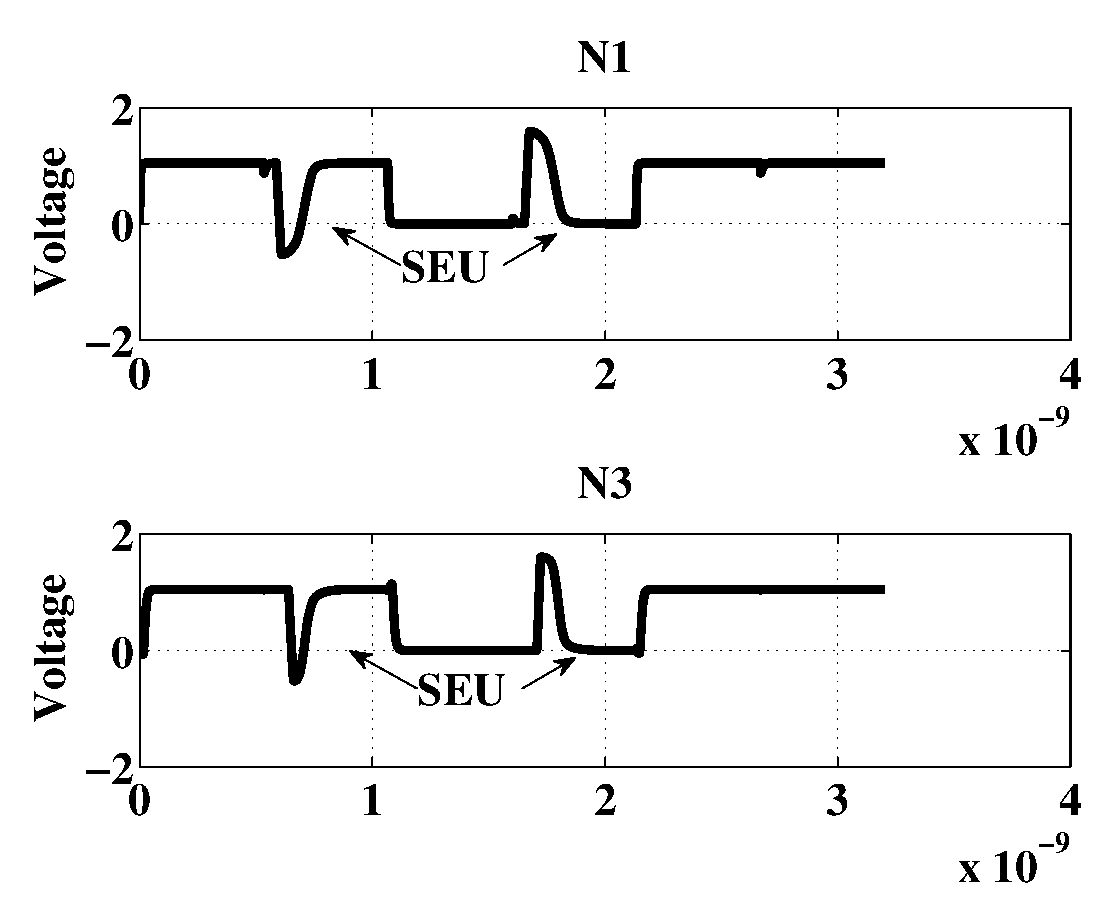
\includegraphics[width=0.5\linewidth]{Figures/WavePlots/n1n3.eps}
	\caption{Node pair n1 and n3 upset and recovery.}
	\label{fig:n1n3}
\end{figure}

\begin{figure}[!htbp]
	\centering
	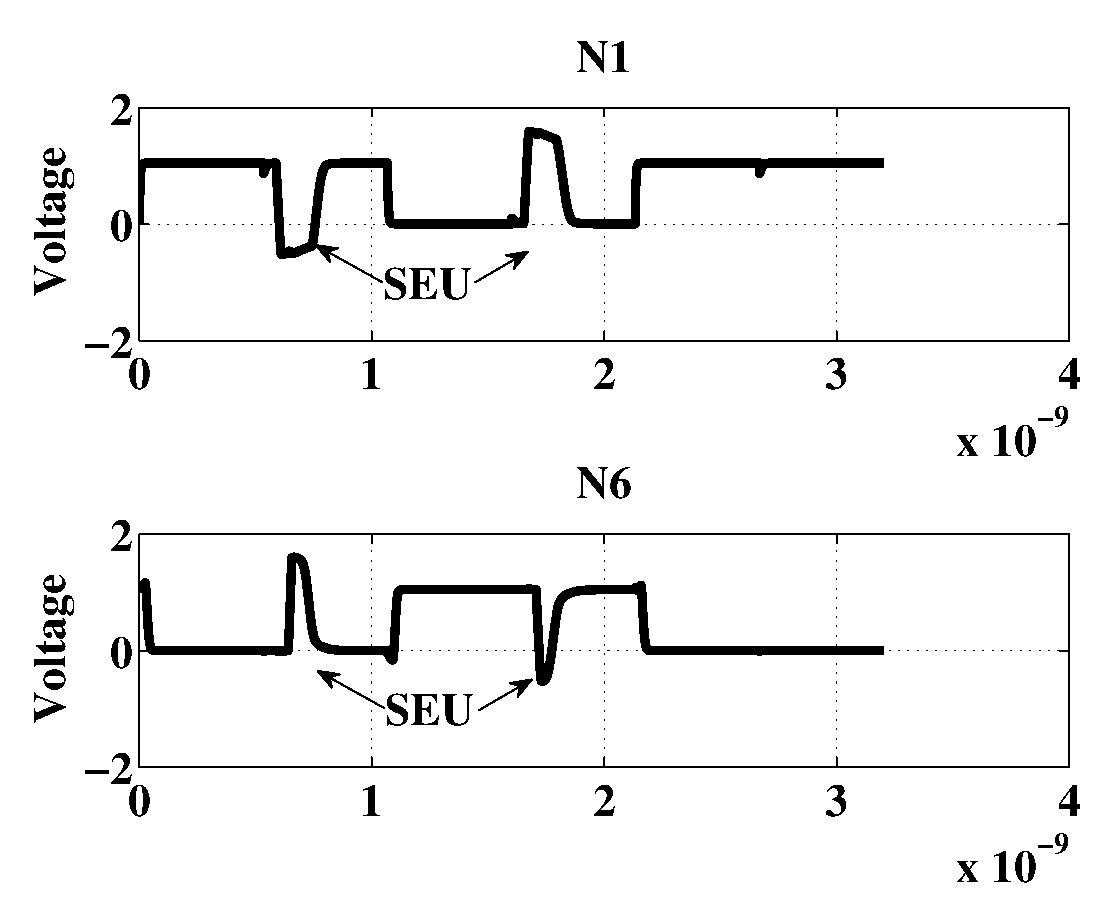
\includegraphics[width=0.5\linewidth]{Figures/WavePlots/n1n6.eps}
	\caption{Node pair n1 and n6 upset and recovery.}
	\label{fig:n1n6}
\end{figure}

\begin{figure}[!htbp]
	\centering
	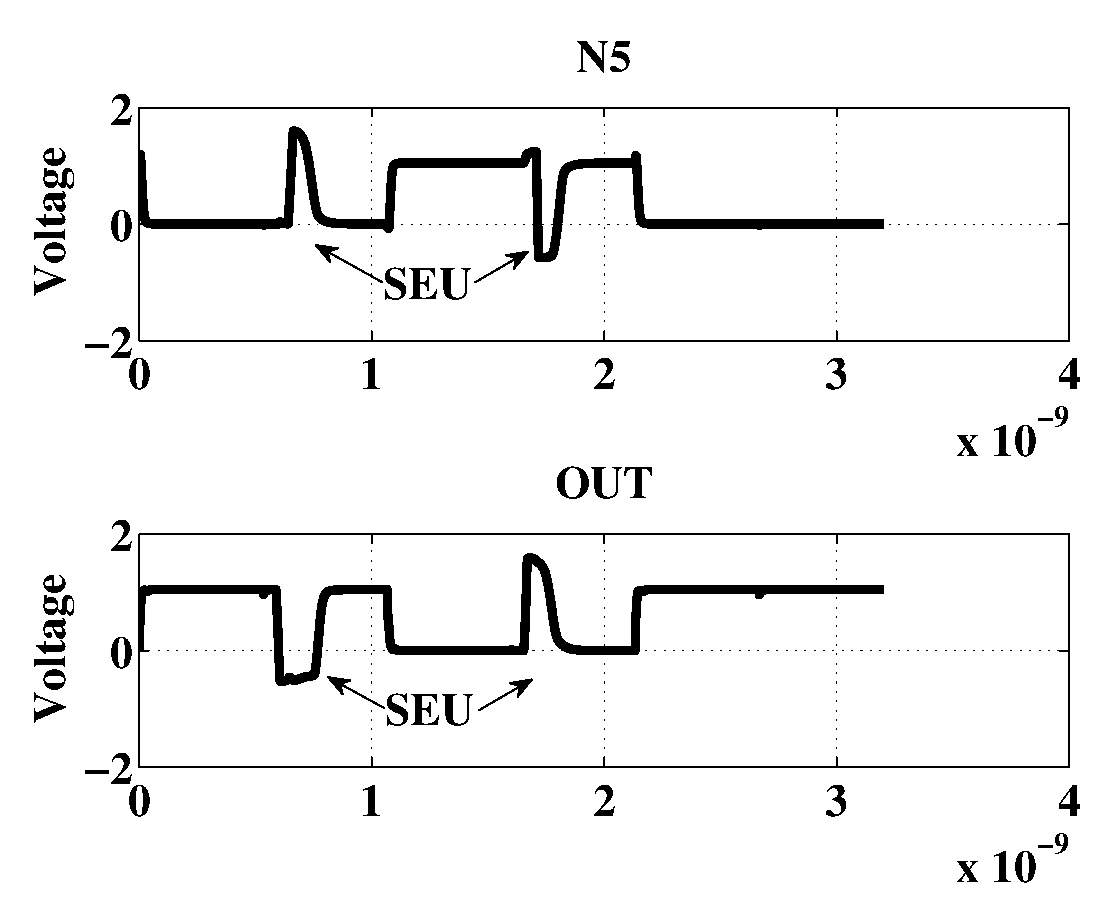
\includegraphics[width=0.5\linewidth]{Figures/WavePlots/n5out.eps}
	\caption{Node pair n5 and out upset and recovery.}
	\label{fig:n3out}
\end{figure}

\begin{figure}
	\centering
	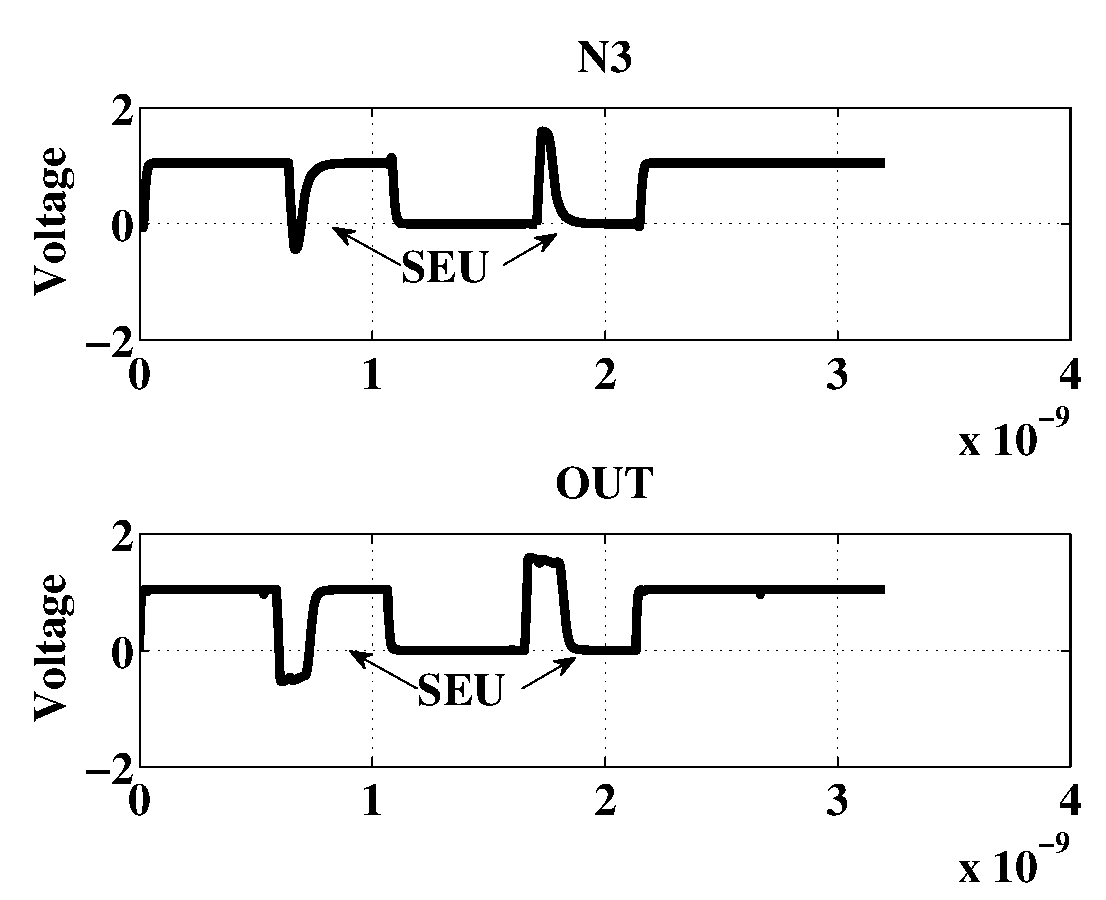
\includegraphics[width=0.5\linewidth]{Figures/WavePlots/n3out.eps}
	\caption{Node pair n3 and out upset and recovery.}
	\label{fig:n5n6}
\end{figure}
